\chapter[Cálculos de la serie de Fourier en hojas de cálculo]{Cálculos de la serie de Fourier en hojas de cálculo}
\label{cp:user-guide}

{
\parindent0pt

En este apartado se presentan los cálculos de la serie de Fourier, desarrollados a partir de las funciones propuestas por el profesor de la materia de Cómputo Paralelo. El objetivo principal de esta fase es llevar a cabo el cálculo de la serie de Fourier utilizando herramientas como Excel, empleando los coeficientes obtenidos en la fase 1.
\vspace{10pt}
%---------------------------------------- Ilse

\newpage
\section{Función resuelta por Castro Paez Ilse Yazbeth}
\label{sec:class-options}
Después de haber realizado los cálculos correrpondientes a la fase 1, se ocupo para continuar la fase 2. Los valores ocupados fueron los siguientes: \(a_0 = 9 - \left(\frac{\pi^2}{3}\right)\), \(a_n =\frac{2\pi (-1)^{n+1}}{n^2}\) y \(b_n = 0\).
La fórmula utilizada se obtiene al sustituir estos coeficientes en la ecuación (\ref{eq:fourier}), quedando de la siguiente forma ya simplificando los términos: 

\begin{equation}
\label{eq:serieFourier-Ilse-simplified}
f(x) = 9 - \left(\frac{\pi^2}{3}\right) + \sum_{n=1}^{\infty} \frac{2\pi (-1)^{n+1}}{n^2} \cos{nx}
\end{equation}
\vspace{10pt}

En la siguiente imagen se muestra la grafica de la función que se obtuvo después de hacer los cálculos correspondientes en Excel y se muestra la gráfica de la función antes de realizar las series de Fourier, para después poder comparar las 2 gráficas obtenidas y analizar los resultados. 


\begin{figure}[H]
    \centering
    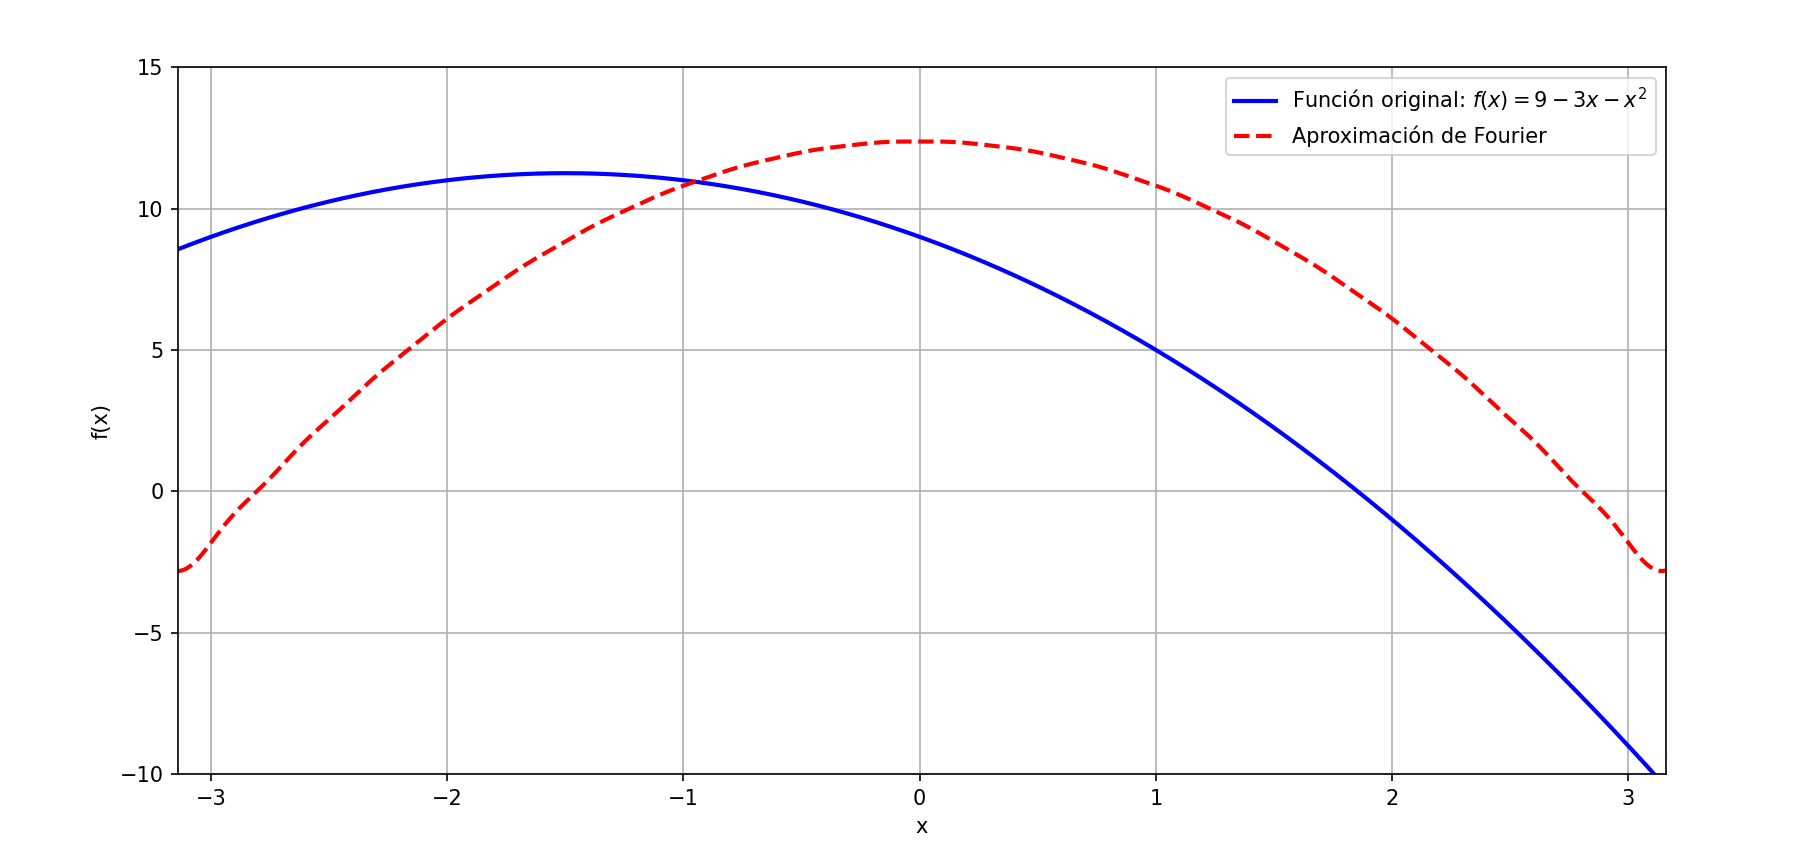
\includegraphics[width=\linewidth]{Figures/fourierIlse/Grafica-Ilse.png}
    \caption[Gráfica de la función \(f(x)=9-3x-x^2\)]{Gráfica de la función  \(f(x)=9-3x-x^2\), resuelto por Castro Paez Ilse Yazbeth}
    \label{fig:figure-ilse-01}
\end{figure}

La función original \( f(x) = 9 - 3x - x^2 \) se graficó en el intervalo \([-3.14, 3.16]\). Esta función es una parábola invertida con un máximo en \( x = -1.5 \) y un valor de \( f(-1.5) = 11.25 \). Las intersecciones con el eje \( x \) se encuentran aproximadamente en \( x = 1.854 \) y \( x = -4.854 \), aunque este último punto está fuera del intervalo graficado.
\vspace{10pt}

La gráfica de la aproximación de Fourier ajustada sigue la forma de la función original, aunque se observan pequeñas diferencias cerca de los extremos del intervalo debido a las discontinuidades introducidas por la extensión periódica.

\vspace{10pt}
La aproximación de Fourier depende del número de términos (n) que se utilicen en la serie. Al comparar las gráficas generadas a partir de los datos, se observa que no coinciden exactamente. Esta diferencia puede atribuirse a varios factores. La función es una parábola, la cual no es una función periódica. La serie de Fourier es más adecuada para aproximar funciones periódicas, por lo que su aplicación en este caso puede introducir errores, especialmente en los extremos del intervalo considerado. Esto contribuye a que las gráficas no coincidan perfectamente.





\newpage
\begin{table}[H]
\begin{center}
\caption{Aproximación de \( f(x) = 9-3x-x^2\) mediante la serie de Fourier}
\resizebox{\textwidth}{!}{%
\begin{tabular}{|c|cccccccccc|c|}
\hline
& \multicolumn{10}{c|}{n} & \\
\cline{2-11}
f(x) & 1 & 2 & 3 & 4 & 5 & 6 & 7 & 8 & 9 & 10 & Suma \\
\hline
-3.14 & 5.710 & -6.283 & -1.571 & -0.698 & -0.393 & -0.251 & -0.175 & -0.128 & -0.098 & -0.078 & -10.737 \\
-2.99 & 5.710 & -6.211 & -1.499 & -0.627 & -0.323 & -0.183 & -0.107 & -0.063 & -0.034 & -0.016 & -10.066 \\
-2.84 & 5.710 & -6.000 & -1.294 & -0.431 & -0.140 & -0.016 & 0.041 & 0.066 & 0.073 & 0.071 & -8.567 \\
-2.69 & 5.710 & -5.653 & -0.973 & -0.150 & 0.092 & 0.159 & 0.158 & 0.128 & 0.087 & 0.047 & -7.091 \\
-2.54 & 5.710 & -5.180 & -0.565 & 0.162 & 0.291 & 0.249 & 0.156 & 0.062 & -0.010 & -0.050 & -5.946 \\
-2.39 & 5.710 & -4.591 & -0.106 & 0.441 & 0.389 & 0.205 & 0.035 & -0.067 & -0.095 & -0.069 & -4.877 \\
-2.24 & 5.710 & -3.898 & 0.362 & 0.633 & 0.351 & 0.051 & -0.112 & -0.128 & -0.059 & 0.020 & -3.723 \\
-2.09 & 5.710 & -3.118 & 0.797 & 0.698 & 0.190 & -0.130 & -0.174 & -0.061 & 0.052 & 0.078 & -2.639 \\
-1.94 & 5.710 & -2.267 & 1.162 & 0.625 & -0.037 & -0.242 & -0.105 & 0.068 & 0.096 & 0.014 & -1.740 \\
-1.79 & 5.710 & -1.366 & 1.422 & 0.427 & -0.251 & -0.224 & 0.044 & 0.128 & 0.018 & -0.071 & -0.910 \\
-1.64 & 5.710 & -0.434 & 1.556 & 0.144 & -0.378 & -0.085 & 0.160 & 0.060 & -0.084 & -0.045 & -0.059 \\
-1.49 & 5.710 & 0.507 & 1.550 & -0.168 & -0.372 & 0.099 & 0.154 & -0.069 & -0.078 & 0.052 & 0.719 \\
-1.34 & 5.710 & 1.437 & 1.406 & -0.446 & -0.237 & 0.230 & 0.032 & -0.128 & 0.027 & 0.068 & 1.347 \\
-1.19 & 5.710 & 2.335 & 1.137 & -0.635 & -0.019 & 0.238 & -0.114 & -0.059 & 0.098 & -0.022 & 1.909 \\
-1.04 & 5.710 & 3.181 & 0.766 & -0.698 & 0.206 & 0.118 & -0.174 & 0.070 & 0.044 & -0.077 & 2.469 \\
-0.89 & 5.710 & 3.955 & 0.326 & -0.622 & 0.359 & -0.065 & -0.102 & 0.128 & -0.066 & -0.012 & 2.955 \\
-0.74 & 5.710 & 4.640 & -0.142 & -0.422 & 0.386 & -0.213 & 0.047 & 0.058 & -0.092 & 0.072 & 3.306 \\
-0.59 & 5.710 & 5.221 & -0.598 & -0.138 & 0.279 & -0.247 & 0.161 & -0.071 & -0.001 & 0.044 & 3.591 \\
-0.44 & 5.710 & 5.685 & -1.001 & 0.173 & 0.074 & -0.148 & 0.153 & -0.128 & 0.091 & -0.053 & 3.866 \\
-0.29 & 5.710 & 6.021 & -1.314 & 0.450 & -0.157 & 0.030 & 0.029 & -0.057 & 0.067 & -0.067 & 4.064 \\
-0.14 & 5.710 & 6.222 & -1.510 & 0.637 & -0.333 & 0.192 & -0.116 & 0.071 & -0.043 & 0.024 & 4.134 \\
0.01 & 5.710 & 6.283 & -1.570 & 0.698 & -0.392 & 0.251 & -0.174 & 0.128 & -0.098 & 0.077 & 4.139 \\
0.16 & 5.710 & 6.203 & -1.491 & 0.619 & -0.315 & 0.175 & -0.100 & 0.056 & -0.028 & 0.010 & 4.131 \\
0.31 & 5.710 & 5.984 & -1.278 & 0.417 & -0.128 & 0.005 & 0.050 & -0.072 & 0.077 & -0.073 & 4.045 \\
0.46 & 5.710 & 5.630 & -0.952 & 0.132 & 0.104 & -0.167 & 0.162 & -0.128 & 0.084 & -0.042 & 3.831 \\
0.61 & 5.710 & 5.150 & -0.540 & -0.179 & 0.300 & -0.250 & 0.152 & -0.055 & -0.016 & 0.054 & 3.554 \\
0.76 & 5.710 & 4.554 & -0.080 & -0.455 & 0.391 & -0.199 & 0.026 & 0.073 & -0.096 & 0.066 & 3.265 \\
0.91 & 5.710 & 3.856 & 0.387 & -0.640 & 0.345 & -0.041 & -0.119 & 0.128 & -0.053 & -0.026 & 2.898 \\
1.06 & 5.710 & 3.072 & 0.820 & -0.698 & 0.179 & 0.139 & -0.174 & 0.054 & 0.058 & -0.077 & 2.397 \\
1.21 & 5.710 & 2.218 & 1.179 & -0.617 & -0.050 & 0.245 & -0.098 & -0.074 & 0.095 & -0.008 & 1.834 \\
1.36 & 5.710 & 1.315 & 1.433 & -0.413 & -0.261 & 0.219 & 0.053 & -0.128 & 0.011 & 0.073 & 1.270 \\
1.51 & 5.710 & 0.382 & 1.559 & -0.127 & -0.381 & 0.075 & 0.163 & -0.053 & -0.087 & 0.040 & 0.624 \\
1.66 & 5.710 & -0.560 & 1.546 & 0.185 & -0.368 & -0.108 & 0.150 & 0.075 & -0.074 & -0.056 & -0.171 \\
1.81 & 5.710 & -1.489 & 1.394 & 0.459 & -0.226 & -0.234 & 0.024 & 0.128 & 0.033 & -0.065 & -1.022 \\
1.96 & 5.710 & -2.384 & 1.118 & 0.642 & -0.005 & -0.234 & -0.121 & 0.052 & 0.098 & 0.027 & -1.852 \\
2.11 & 5.710 & -3.226 & 0.743 & 0.697 & 0.217 & -0.108 & -0.174 & -0.076 & 0.038 & 0.077 & -2.773 \\
2.26 & 5.710 & -3.996 & 0.300 & 0.614 & 0.364 & 0.075 & -0.095 & -0.127 & -0.071 & 0.006 & -3.878 \\
2.41 & 5.710 & -4.675 & -0.169 & 0.408 & 0.384 & 0.219 & 0.055 & -0.051 & -0.089 & -0.074 & -5.025 \\
2.56 & 5.710 & -5.250 & -0.623 & 0.121 & 0.269 & 0.245 & 0.164 & 0.077 & 0.006 & -0.039 & -6.086 \\
2.71 & 5.710 & -5.707 & -1.021 & -0.190 & 0.061 & 0.139 & 0.149 & 0.127 & 0.093 & 0.057 & -7.267 \\
2.86 & 5.710 & -6.036 & -1.328 & -0.463 & -0.169 & -0.041 & 0.021 & 0.050 & 0.062 & 0.064 & -8.781 \\
3.01 & 5.710 & -6.229 & -1.517 & -0.644 & -0.340 & -0.199 & -0.123 & -0.078 & -0.049 & -0.029 & -10.223 \\
3.16 & 5.710 & -6.282 & -1.570 & -0.697 & -0.392 & -0.250 & -0.173 & -0.127 & -0.097 & -0.077 & -10.727 \\
\hline
\end{tabular}
}
\end{center}
\end{table}








\section{Función resuelta por Catonga Daniel Isaí}
\label{sec:class-options}

Para realizar los cálculos de la serie de Fourier, se utilizan los valores obtenidos en la fase 1, los coeficientes se muestran a continuación:
\[
a_0 = 12, \quad a_n = 0, \quad b_n = \frac{4x}{n}(-1)^n.
\]
La fórmula a utilizar se obtiene al sustituir estos coeficientes en la ecuación (\ref{eq:fourier}), quedando de la siguiente forma:

\begin{equation}
\label{eq:serieFourier-Daniel}
f(x) = \frac{12}{2} + \sum_{n=1}^{\infty} \frac{4}{n}(-1)^n \sin(nx)
\end{equation}

Simplificando (\ref{eq:serieFourier-Daniel}), se obtiene:
\begin{equation}
\label{eq:serieFourier-Daniel-simplified}
f(x) = 6 + \sum_{n=1}^{\infty} \frac{4}{n}(-1)^n \sin(nx)
\end{equation}

A continuación, se presenta la función original que se desea resolver. Recordemos que la función original es \(f(x)=6-2x\), y su representación gráfica se muestra en la figura \ref{fig:figure-danielexcel-01}.

\vspace{10pt}

\begin{figure}[H]
    \centering
    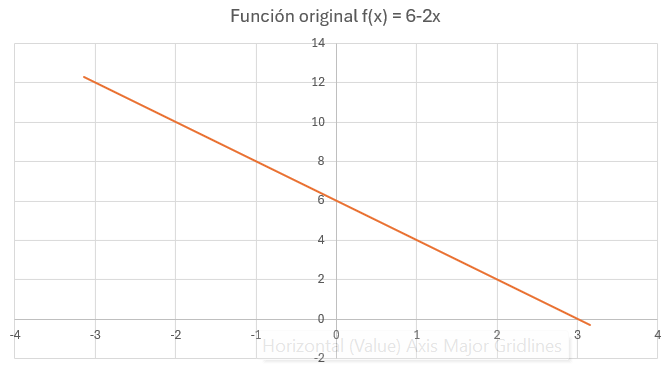
\includegraphics[width=\linewidth]{Figures/fourierDaniel/Funcion original.png}
    \caption[Gráfica en Excel de la función original \(f(x)=6-2x\)]{Gráfica en Excel de la función original \(f(x)=6 - 2x\)}  % Corregido
    \label{fig:figure-danielexcel-01}
\end{figure}

\vspace{10pt}

A continuación, se presenta la tabla \ref{tab:table-daniel-01}, que muestra los cálculos obtenidos a partir de 10 iteraciones de la serie de Fourier aplicada en la ecuación (\ref{eq:serieFourier-Daniel-simplified}), para \(x\) en el intervalor de \([-\pi,\pi]\). En esta tabla se detallan los resultados de dicha aplicación.

\newpage
\begin{table}[H]
\begin{center}
\caption{Aproximación de \( f(x) = 6 - 2x \) mediante la serie de Fourier}
\label{tab:table-daniel-01}
\resizebox{\textwidth}{!}{%
\begin{tabular}{|c|cccccccccc|c|}
\hline
& \multicolumn{10}{c|}{n} & \\
\cline{2-11}
f(x) & 1 & 2 & 3 & 4 & 5 & 6 & 7 & 8 & 9 & 10 & Suma \\
\hline
-3.14 & 0.006 & 0.006 & 0.006 & 0.006 & 0.006 & 0.006 & 0.006 & 0.006 & 0.006 & 0.006 & 6.064 \\
-2.99 & 0.604 & 0.597 & 0.586 & 0.570 & 0.550 & 0.526 & 0.499 & 0.468 & 0.435 & 0.399 & 11.234 \\
-2.84 & 1.188 & 1.135 & 1.048 & 0.934 & 0.798 & 0.648 & 0.490 & 0.333 & 0.184 & 0.050 & 12.809 \\
-2.69 & 1.746 & 1.571 & 1.302 & 0.972 & 0.618 & 0.279 & -0.011 & -0.227 & -0.354 & -0.392 & 11.504 \\
-2.54 & 2.264 & 1.866 & 1.297 & 0.671 & 0.107 & -0.301 & -0.501 & -0.497 & -0.339 & -0.106 & 10.460 \\
-2.39 & 2.731 & 1.995 & 1.033 & 0.135 & -0.462 & -0.653 & -0.488 & -0.134 & 0.206 & 0.377 & 10.741 \\
-2.24 & 3.137 & 1.946 & 0.564 & -0.448 & -0.783 & -0.511 & 0.016 & 0.401 & 0.429 & 0.159 & 10.910 \\
-2.09 & 3.473 & 1.723 & -0.018 & -0.875 & -0.684 & 0.018 & 0.503 & 0.424 & -0.018 & -0.355 & 10.192 \\
-1.94 & 3.730 & 1.346 & -0.596 & -0.996 & -0.217 & 0.533 & 0.485 & -0.093 & -0.437 & -0.209 & 9.546 \\
-1.79 & 3.904 & 0.849 & -1.055 & -0.769 & 0.366 & 0.645 & -0.021 & -0.492 & -0.174 & 0.325 & 9.579 \\
-1.64 & 3.990 & 0.276 & -1.305 & -0.273 & 0.753 & 0.269 & -0.506 & -0.263 & 0.361 & 0.255 & 9.558 \\
-1.49 & 3.987 & -0.322 & -1.294 & 0.318 & 0.736 & -0.311 & -0.482 & 0.301 & 0.332 & -0.289 & 8.975 \\
-1.34 & 3.894 & -0.891 & -1.026 & 0.798 & 0.324 & -0.655 & 0.026 & 0.481 & -0.216 & -0.296 & 8.438 \\
-1.19 & 3.713 & -1.380 & -0.554 & 0.999 & -0.262 & -0.504 & 0.508 & 0.048 & -0.426 & 0.247 & 8.389 \\
-1.04
& 3.450 & -1.746 & 0.029 & 0.851 & -0.707 & 0.029 & 0.480 & -0.447 & 0.029 & 0.331 & 8.299 \\
-0.89
& 3.108 & -1.956 & 0.606 & 0.406 & -0.773 & 0.540 & -0.030 & -0.371 & 0.439 & -0.200 & 7.768 \\
-0.74
& 2.697 & -1.992 & 1.062 & -0.181 & -0.424 & 0.642 & -0.510 & 0.178 & 0.164 & -0.359 & 7.277 \\
-0.59
& 2.225 & -1.849 & 1.307 & -0.704 & 0.152 & 0.259 & -0.477 & 0.500 & -0.367 & 0.150 & 7.195 \\
-0.44
& 1.704 & -1.541 & 1.292 & -0.982 & 0.647 & -0.321 & 0.035 & 0.185 & -0.324 & 0.381 & 7.074 \\
-0.29
& 1.144 & -1.096 & 1.019 & -0.917 & 0.794 & -0.657 & 0.512 & -0.366 & 0.225 & -0.096 & 6.563 \\
-0.14
& 0.558 & -0.553 & 0.544 & -0.531 & 0.515 & -0.496 & 0.475 & -0.450 & 0.423 & -0.394 & 6.090 \\
0.01
& -0.040 & 0.040 & -0.040 & 0.040 & -0.040 & 0.040 & -0.040 & 0.040 & -0.040 & 0.040 & 6.000 \\
0.16
& -0.637 & 0.629 & -0.616 & 0.597 & -0.574 & 0.546 & -0.514 & 0.479 & -0.441 & 0.400 & 5.869 \\
0.31
& -1.220 & 1.162 & -1.069 & 0.946 & -0.800 & 0.639 & -0.472 & 0.307 & -0.153 & 0.017 & 5.357 \\
0.46
& -1.776 & 1.591 & -1.309 & 0.964 & -0.597 & 0.248 & 0.045 & -0.256 & 0.374 & -0.397 & 4.886 \\
0.61
& -2.291 & 1.878 & -1.289 & 0.645 & -0.073 & -0.330 & 0.516 & -0.493 & 0.317 & -0.073 & 4.807 \\
0.76
& -2.756 & 1.997 & -1.012 & 0.101 & 0.489 & -0.659 & 0.469 & -0.101 & -0.235 & 0.387 & 4.682 \\
0.91
& -3.158 & 1.938 & -0.533 & -0.478 & 0.789 & -0.489 & -0.050 & 0.420 & -0.420 & 0.128 & 4.148 \\
1.06
& -3.489 & 1.706 & 0.051 & -0.890 & 0.666 & 0.051 & -0.518 & 0.405 & 0.051 & -0.369 & 3.663 \\
1.21
& -3.742 & 1.321 & 0.626 & -0.992 & 0.185 & 0.552 & -0.466 & -0.126 & 0.442 & -0.180 & 3.619 \\
1.36
& -3.911 & 0.818 & 1.075 & -0.747 & -0.395 & 0.636 & 0.054 & -0.497 & 0.142 & 0.344 & 3.520 \\
1.51
& -3.993 & 0.243 & 1.311 & -0.241 & -0.763 & 0.238 & 0.520 & -0.234 & -0.380 & 0.228 & 2.931 \\
1.66
& -3.984 & -0.355 & 1.286 & 0.349 & -0.722 & -0.340 & 0.464 & 0.327 & -0.309 & -0.311 & 2.405 \\
1.81
& -3.886 & -0.921 & 1.005 & 0.817 & -0.293 & -0.661 & -0.059 & 0.471 & 0.244 & -0.273 & 2.445 \\
1.96
& -3.701 & -1.404 & 0.523 & 1.000 & 0.293 & -0.481 & -0.522 & 0.014 & 0.416 & 0.273 & 2.410 \\
2.11
& -3.432 & -1.762 & -0.062 & 0.833 & 0.722 & 0.062 & -0.461 & -0.461 & -0.062 & 0.311 & 1.687 \\
2.26
& -3.087 & -1.963 & -0.636 & 0.375 & 0.763 & 0.559 & 0.064 & -0.348 & -0.443 & -0.229 & 1.056 \\
2.41
& -2.672 & -1.988 & -1.082 & -0.214 & 0.395 & 0.632 & 0.524 & 0.209 & -0.132 & -0.343 & 1.329 \\
2.56
& -2.197 & -1.836 & -1.313 & -0.728 & -0.185 & 0.227 & 0.458 & 0.499 & 0.385 & 0.180 & 1.490 \\
2.71
& -1.673 & -1.520 & -1.283 & -0.988 & -0.666 & -0.350 & -0.069 & 0.153 & 0.301 & 0.369 & 0.274 \\
2.86
& -1.112 & -1.068 & -0.997 & -0.903 & -0.789 & -0.662 & -0.526 & -0.388 & -0.254 & -0.128 & -0.827 \\
3.01
& -0.525 & -0.520 & -0.513 & -0.502 & -0.489 & -0.473 & -0.455 & -0.434 & -0.412 & -0.387 & 1.289 \\
3.16
& 0.074 & 0.074 & 0.074 & 0.074 & 0.074 & 0.073 & 0.073 & 0.073 & 0.073 & 0.073 & 6.735 \\
\hline
\end{tabular}
}
\end{center}
\end{table}

\newpage
\begin{minipage}{\textwidth}
    Al graficar los valores de la tabla \ref{tab:table-daniel-01}, obtenemos la aproximación de la función \(f(x)=6-2x\) mediante la serie de Fourier, se muestra en la figura \ref{fig:figure-danielexcel-02}. Esta serie corresponde a la suma de las componentes armónicas que aproximan la función original en el intervalo \([-\pi,\pi]\).
    
    % Segunda Gráfica - gráfica de la función de Fourier %
    \begin{figure}[H]
        \centering
        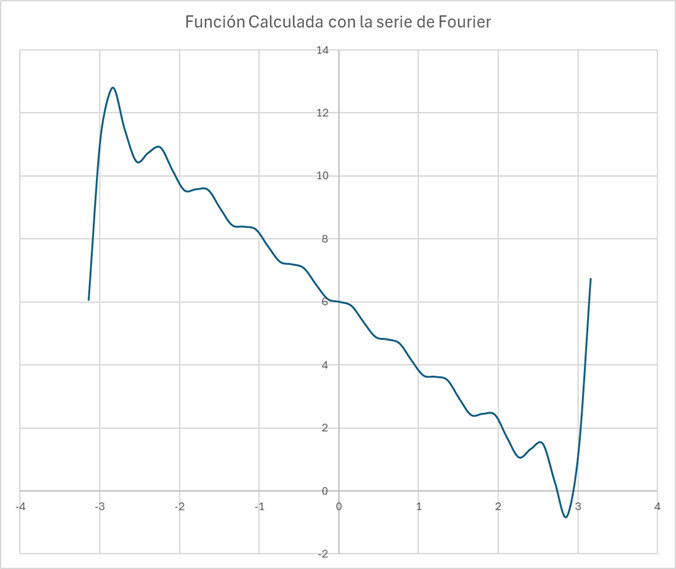
\includegraphics[width=0.9\linewidth,height=0.3\textheight]{Figures/fourierDaniel/Funcion Calculada.png}
        \caption[Gráfica de la aproximación de \( f(x) = 6 - 2x \) mediante la serie de Fourier]{Gráfica de la aproximación de la función \( f(x) = 6 - 2x \) obtenida a través de la serie de Fourier, calculada por Catonga Tecla Daniel Isaí}
        \label{fig:figure-danielexcel-02}
    \end{figure}
    

    Al comparar las gráficas mostradas en la figura \ref{fig:figure-danielexcel-03}, se observa que la serie de Fourier se ajusta progresivamente a la función original. A medida que se aumentan las iteraciones, la aproximación se vuelve cada vez más precisa.

    % Tercer Gráfica - gráficas comparativas %
    \begin{figure}[H]
    \centering
        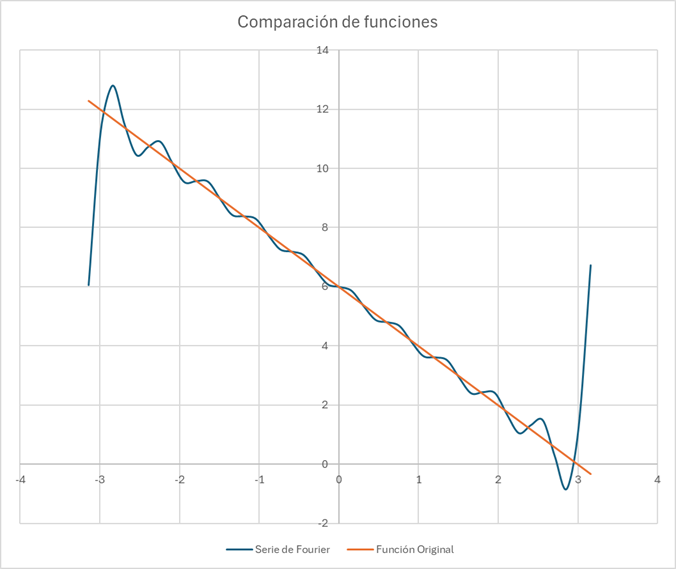
\includegraphics[width=0.9\linewidth, height=0.3\textheight]{Figures/fourierDaniel/Comparacion.png}
        \caption[Comparación entre la función original y la serie de Fourier]{Comparación la función original y la serie de Fourier, resuelto por Catonga Tecla Daniel Isaí}
        \label{fig:figure-danielexcel-03}
    \end{figure}
    
\end{minipage}

\section{Función resuelta por Olguin Castillo Victor Manuel}
\label{sec:class-options}

La serie de Fourier para la función \( f(x) = x^2 - 3x - 3 \) se construye a partir de los coeficientes calculados previamente. Estos coeficientes son: 
\[
a_0 = \frac{2\pi^2}{3} - 6, \quad a_n = \frac{4(-1)^n}{n^2}, \quad b_n = \frac{6(-1)^n}{n}.
\]
Sustituyendo estos valores en la expresión general de la serie de Fourier, obtenemos la siguiente representación de la función:

\begin{equation}
\label{eq:serieFourier-x2-3x-3}
f(x) = \frac{\pi^2}{3} - 3 + \sum_{n=1}^{\infty} \left( \frac{4(-1)^n}{n^2} \cos{nx} + \frac{6(-1)^n}{n} \sin{nx} \right).
\end{equation}

Esta serie combina términos cosenoidales y sinusoidales, cuyas amplitudes están determinadas por los coeficientes \( a_n \) y \( b_n \), respectivamente.
\\ 

Representación gráfica obtenida en Excel de la función \(f(x) = x^2 - 3x - 3\) y su aproximación mediante series de Fourier en (\ref{fig:figure-manuel-04}). 

% En la sección de Olguin Castillo:
\begin{figure}[H]
    \centering
    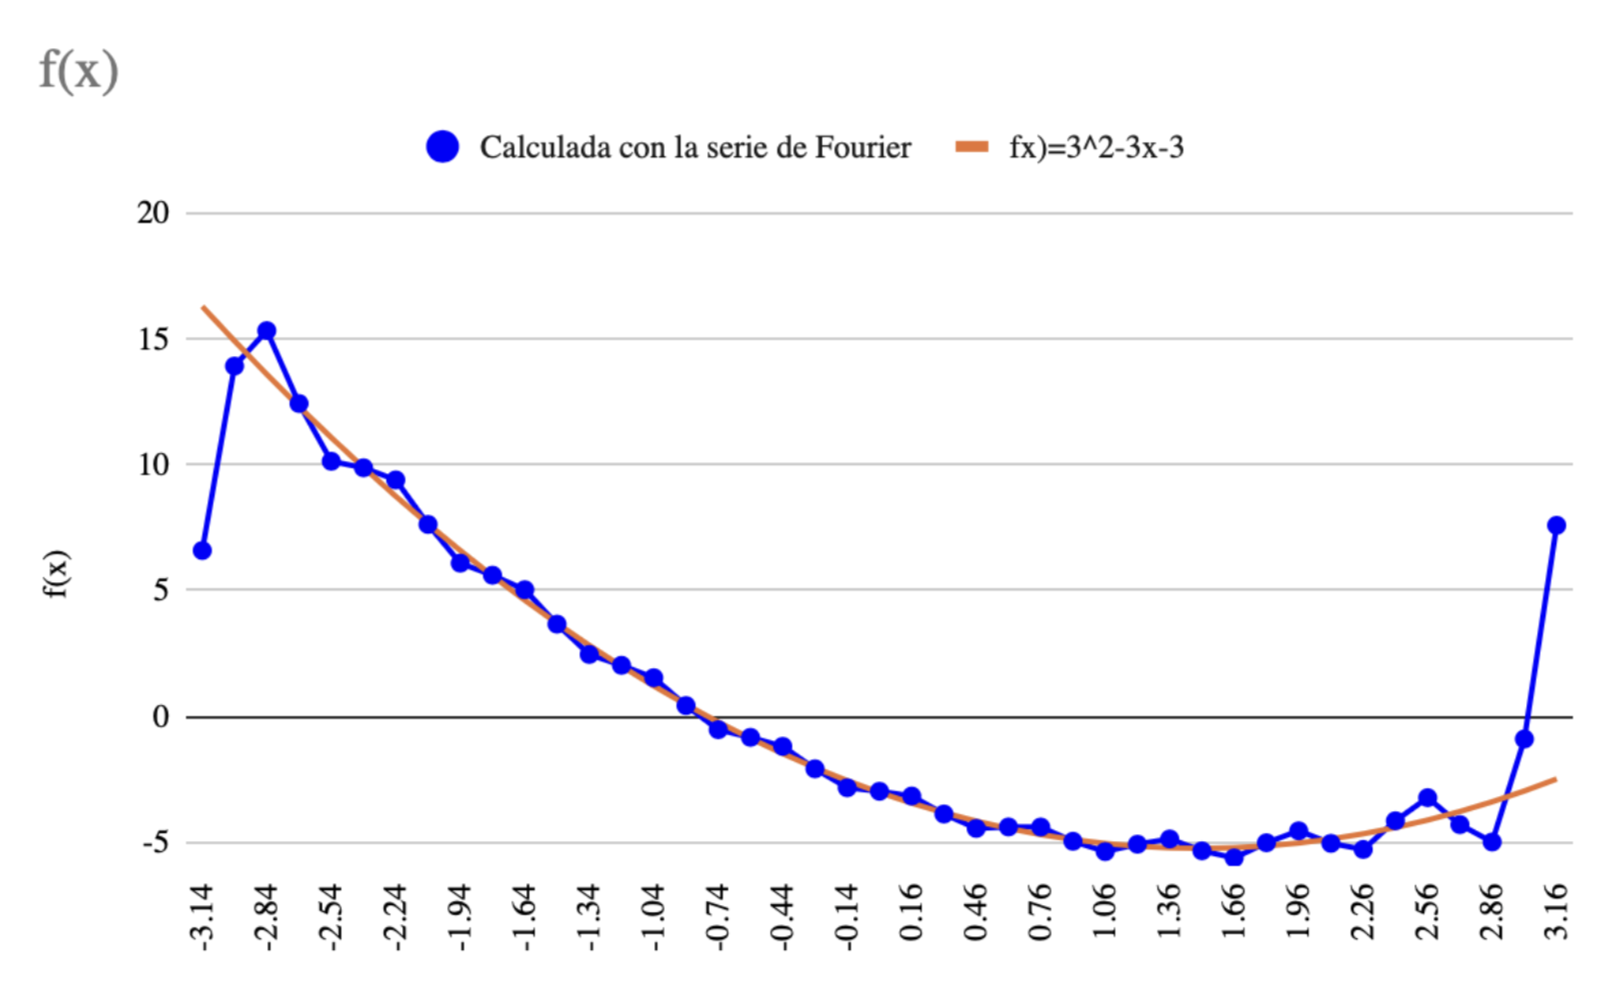
\includegraphics[width=\linewidth]{Figures/fourierManuel/graficaExcel-Manuel.png}
    \caption[Gráfica en Excel de la función \(f(x)=x^2 - 3x - 3\)]{Gráfica en Excel de la función  \(f(x)=x^2 - 3x - 3\), resuelto por Olguin Castillo Victor Manuel}  % Corregido
    \label{fig:figure-manuel-04}
\end{figure}
Posteriormente, se llevó a cabo el cálculo de la serie de Fourier con al menos 10 iteraciones, obteniendo una matriz de valores, mostrada a continuación.
\newpage
\begin{table}[H]
\centering
\caption{Aproximación de \( f(x) = x^2 - 3x -3\) mediante la serie de Fourier}
\resizebox{\textwidth}{!}{%
\begin{tabular}{|c|cccccccccc|c|c|}
\hline
& \multicolumn{10}{c|}{n} & \\
\cline{2-11}
f(x) & 0 & 1 & 2 & 3 & 4 & 5 & 6 & 7 & 8 & 9 & Suma \\
\hline
-3.140 & 0.290 & 4.010 & 2.480 & 0.643 & -0.933 & 0.245 & 0.719 & -0.836 & -0.324 & 0.615 & 6.929 \\
-2.990 & 0.290 & 4.860 & 2.480 & -1.616 & -0.933 & 1.205 & 0.719 & -0.670 & -0.324 & -0.214 & 5.819 \\
-2.840 & 0.290 & 5.602 & 2.480 & 1.983 & -0.933 & 0.704 & 0.719 & 0.820 & -0.324 & -0.616 & 10.745 \\
-2.690 & 0.290 & 6.217 & 2.480 & -0.044 & -0.933 & 0.104 & 0.719 & -0.631 & -0.324 & -0.419 & 7.481 \\
-2.540 & 0.290 & 6.694 & 2.480 & -2.034 & -0.933 & -0.695 & 0.719 & -0.860 & -0.324 & 0.656 & 6.014 \\
-2.390 & 0.290 & 7.019 & 2.480 & -1.343 & -0.933 & 0.356 & 0.719 & -0.452 & -0.324 & -0.502 & 7.332 \\
-2.240 & 0.290 & 7.187 & 2.480 & -0.428 & -0.933 & 1.097 & 0.719 & -0.858 & -0.324 & 0.655 & 9.906 \\
-2.090 & 0.290 & 7.194 & 2.480 & -0.388 & -0.933 & 1.177 & 0.719 & -0.763 & -0.324 & 0.324 & 9.798 \\
-1.940 & 0.290 & 7.039 & 2.480 & -1.248 & -0.933 & -0.212 & 0.719 & 0.847 & -0.324 & -0.660 & 8.019 \\
-1.790 & 0.290 & 6.726 & 2.480 & -2.048 & -0.933 & -0.765 & 0.719 & -0.735 & -0.324 & 0.173 & 5.603 \\
-1.640 & 0.290 & 6.262 & 2.480 & -0.318 & -0.933 & 1.203 & 0.719 & -0.680 & -0.324 & -0.158 & 8.562 \\
-1.490 & 0.290 & 5.658 & 2.480 & 2.041 & -0.933 & 0.958 & 0.719 & -0.425 & -0.324 & -0.383 & 10.102 \\
-1.340 & 0.290 & 4.926 & 2.480 & -1.338 & -0.933 & 0.328 & 0.719 & -0.589 & -0.324 & -0.583 & 4.997 \\
-1.190 & 0.290 & 4.084 & 2.480 & 0.198 & -0.933 & -1.092 & 0.719 & 0.821 & -0.324 & -0.619 & 5.645 \\
-1.040 & 0.290 & 3.149 & 2.480 & 0.492 & -0.933 & -0.632 & 0.719 & -0.798 & -0.324 & 0.490 & 4.955 \\
-0.890 & 0.290 & 2.145 & 2.480 & -0.741 & -0.933 & -0.503 & 0.719 & -0.242 & -0.324 & 0.574 & 3.486 \\
-0.740 & 0.290 & 1.092 & 2.480 & 0.708 & -0.933 & 0.611 & 0.719 & 0.811 & -0.324 & -0.594 & 4.881 \\
-0.590 & 0.290 & 0.014 & 2.480 & -0.530 & -0.933 & 0.705 & 0.719 & 0.817 & -0.324 & -0.609 & 2.651 \\
-0.440 & 0.290 & -1.063 & 2.480 & 0.347 & -0.933 & -1.158 & 0.719 & 0.851 & -0.324 & -0.663 & 0.566 \\
-0.290 & 0.290 & -2.117 & 2.480 & -0.306 & -0.933 & 1.193 & 0.719 & -0.715 & -0.324 & 0.053 & 0.360 \\
-0.140 & 0.290 & -3.124 & 2.480 & 0.552 & -0.933 & -0.300 & 0.719 & 0.780 & -0.324 & -0.486 & -0.325 \\
0.010 & 0.290 & -4.060 & 2.480 & -1.166 & -0.933 & -0.668 & 0.719 & -0.853 & -0.324 & 0.648 & -3.846 \\
0.160 & 0.290 & -4.905 & 2.480 & 1.918 & -0.933 & 0.358 & 0.719 & -0.444 & -0.324 & -0.472 & -1.292 \\
0.310 & 0.290 & -5.640 & 2.480 & -1.716 & -0.933 & 1.005 & 0.719 & -0.645 & -0.324 & -0.349 & -5.091 \\
0.460 & 0.290 & -6.248 & 2.480 & -0.653 & -0.933 & 0.009 & 0.719 & -0.138 & -0.324 & 0.614 & -4.162 \\
0.610 & 0.290 & -6.716 & 2.480 & 1.806 & -0.933 & -0.313 & 0.719 & 0.745 & -0.324 & -0.317 & -2.542 \\
0.760 & 0.290 & -7.033 & 2.480 & 1.836 & -0.933 & -0.134 & 0.719 & 0.645 & -0.324 & 0.265 & -2.169 \\
0.910 & 0.290 & -7.192 & 2.480 & 1.213 & -0.933 & 0.102 & 0.719 & -0.622 & -0.324 & -0.462 & -4.708 \\
1.060 & 0.290 & -7.190 & 2.480 & 1.225 & -0.933 & 0.031 & 0.719 & -0.261 & -0.324 & 0.509 & -3.434 \\
1.210 & 0.290 & -7.026 & 2.480 & 1.855 & -0.933 & -0.020 & 0.719 & 0.039 & -0.324 & -0.278 & -3.176 \\
1.360 & 0.290 & -6.704 & 2.480 & 1.771 & -0.933 & -0.511 & 0.719 & -0.290 & -0.324 & 0.382 & -3.099 \\
1.510 & 0.290 & -6.232 & 2.480 & -0.745 & -0.933 & -0.530 & 0.719 & -0.391 & -0.324 & -0.200 & -5.846 \\
1.660 & 0.290 & -5.620 & 2.480 & -1.646 & -0.933 & 1.175 & 0.719 & -0.768 & -0.324 & 0.354 & -4.251 \\
1.810 & 0.290 & -4.881 & 2.480 & 1.964 & -0.933 & 0.610 & 0.719 & 0.810 & -0.324 & -0.590 & 0.166 \\
1.960 & 0.290 & -4.034 & 2.480 & -1.296 & -0.933 & 0.076 & 0.719 & -0.504 & -0.324 & -0.647 & -4.152 \\
2.110 & 0.290 & -3.095 & 2.480 & 0.719 & -0.933 & 0.671 & 0.719 & 0.858 & -0.324 & -0.667 & 0.739 \\
2.260 & 0.290 & -2.087 & 2.480 & -0.490 & -0.933 & 0.890 & 0.719 & -0.034 & -0.324 & 0.151 & 0.683 \\
2.410 & 0.290 & -1.032 & 2.480 & 0.536 & -0.933 & -0.392 & 0.719 & 0.405 & -0.324 & 0.367 & 2.136 \\
2.560 & 0.290 & 0.046 & 2.480 & -0.717 & -0.933 & -0.368 & 0.719 & 0.528 & -0.324 & 0.664 & 2.406 \\
2.710 & 0.290 & 1.123 & 2.480 & 0.886 & -0.933 & 1.197 & 0.719 & -0.702 & -0.324 & -0.026 & 4.731 \\
2.860 & 0.290 & 2.175 & 2.480 & -0.911 & -0.933 & -1.161 & 0.719 & 0.848 & -0.324 & -0.661 & 2.543 \\
3.010 & 0.290 & 3.178 & 2.480 & 0.661 & -0.933 & 0.351 & 0.719 & -0.480 & -0.324 & -0.596 & 5.366 \\
3.160 & 0.290 & 4.110 & 2.480 & 0.038 & -0.933 & -0.382 & 0.719 & 0.458 & -0.324 & 0.581 & 7.057 \\
\hline
\end{tabular}
}
\end{table}

%-------------------Hariel-----------------------------
\section{Función resuelta por Hariel Padilla Sanchez}
\label{sec:class-options}


La serie de Fourier para la función \( f(x) = 6-4x \) se obtiene a partir del cálculo de sus coeficientes, los cuales se presentan a continuación:
\[
a_0 = 12, \quad a_n = 0, \quad b_n = \frac{8(-1)^n}{n}.
\]
Al sustituir estos coeficientes en la expresión general de la serie de Fourier, se obtiene la siguiente forma:

\begin{equation}
\label{eq:serieFourier-6-4x}
f(x) = 6 + \sum_{n=1}^{\infty} \left( \frac{8(-1)^n }{n} * \sin{nx} \right).
\end{equation}

Representación gráfica obtenida en Excel de la función \(f(x) =6-4x\) como muestra el grafico (\ref{fig:figure-hariel-03}). 

% Grafica sola de la funcion
\begin{figure}[H]
    \centering
    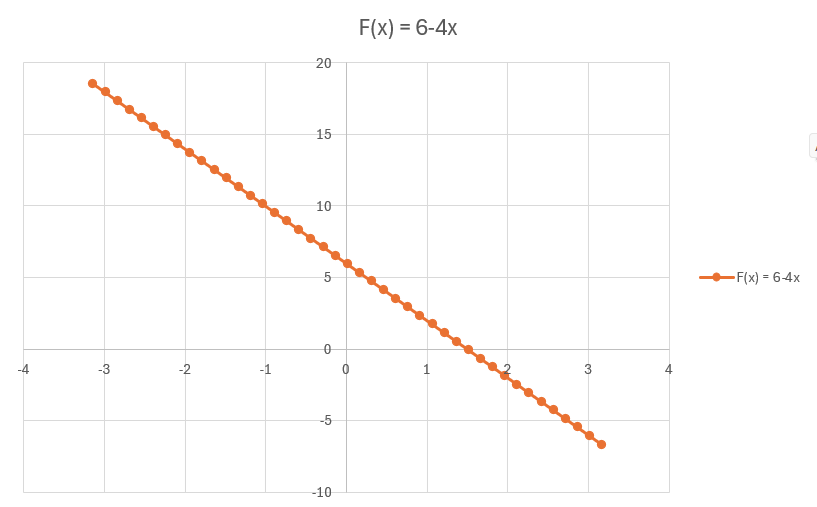
\includegraphics[width=\linewidth]{Figures/fourierHariel/fase2/funcion_sola.png}
    \caption[Gráfica en Excel de la función \(f(x)=6-4x\)]{Gráfica en Excel de la función  \(f(x)=6-4x\), resuelto por Padilla Sanchez Hariel}
    \label{fig:figure-hariel-03}
\end{figure}

Posteriormente, se llevó a cabo el cálculo de la serie de Fourier con al menos 10 iteraciones, obteniendo una matriz de valores como la que se presenta en la Tabla (\ref{tab:tabla-hariel-01})Dichos valores permiten observar la aproximación de la serie a la función dentro del intervalo de interés.

%\begin{tabular}{|c|cccccccccc|c|c|}

\begin{table}[H]
    \centering
    \caption{Aproximación de \( f(x) = 6 - 4x \) mediante la serie de Fourier}
    \resizebox{\textwidth}{!}{%
    \begin{tabular}{|c|cccccccccc|c|c|}
    \hline
    & \multicolumn{10}{c|}{n} & \\
    \cline{2-11}
    f(x) & 0 & 1 & 2 & 3 & 4 & 5 & 6 & 7 & 8 & 9 & Suma \\
    \hline
        -3.14 & 6 & 0.013 & 0.013 & 0.013 & 0.013 & 0.013 & 0.013 & 0.013 & 0.013 & 0.013 & 6.115 \\ 
        -2.99 & 6 & 1.208 & 1.194 & 1.171 & 1.140 & 1.100 & 1.052 & 0.998 & 0.937 & 0.870 & 15.670 \\ 
        -2.84 & 6 & 2.376 & 2.269 & 2.097 & 1.869 & 1.597 & 1.296 & 0.980 & 0.666 & 0.368 & 19.518 \\ 
        -2.69 & 6 & 3.491 & 3.141 & 2.605 & 1.945 & 1.237 & 0.558 & -0.022 & -0.454 & -0.709 & 17.792 \\ 
        -2.54 & 6 & 4.528 & 3.733 & 2.594 & 1.342 & 0.213 & -0.601 & -1.002 & -0.995 & -0.679 & 15.132 \\ 
        -2.39 & 6 & 5.462 & 3.991 & 2.067 & 0.270 & -0.925 & -1.306 & -0.975 & -0.267 & 0.411 & 14.728 \\ 
        -2.24 & 6 & 6.275 & 3.892 & 1.128 & -0.896 & -1.567 & -1.022 & 0.032 & 0.801 & 0.859 & 15.502 \\
        -2.09 & 6 & 6.946 & 3.446 & -0.035 & -1.749 & -1.368 & 0.035 & 1.007 & 0.848 & -0.035 & 15.095 \\ 
        -1.94 & 6 & 7.461 & 2.692 & -1.191 & -1.991 & -0.435 & 1.066 & 0.970 & -0.187 & -0.874 & 13.511 \\
        -1.79 & 6 & 7.809 & 1.698 & -2.111 & -1.537 & 0.731 & 1.290 & -0.042 & -0.983 & -0.348 & 12.507 \\ 
        -1.64 & 6 & 7.981 & 0.552 & -2.609 & -0.547 & 1.505 & 0.538 & -1.011 & -0.526 & 0.722 & 12.605 \\ 
        -1.49 & 6 & 7.974 & -0.644 & -2.589 & 0.635 & 1.471 & -0.621 & -0.965 & 0.602 & 0.664 & 12.528 \\ 
        -1.34 & 6 & 7.788 & -1.781 & -2.053 & 1.595 & 0.648 & -1.310 & 0.051 & 0.962 & -0.431 & 11.469 \\ 
        -1.19 & 6 & 7.427 & -2.760 & -1.108 & 1.998 & -0.523 & -1.008 & 1.016 & 0.095 & -0.853 & 10.284 \\
        -1.04 & 6 & 6.899 & -3.493 & 0.058 & 1.703 & -1.414 & 0.058 & 0.960 & -0.893 & 0.058 & 9.935 \\ 
        -0.89 & 6 & 6.217 & -3.913 & 1.211 & 0.813 & -1.545 & 1.079 & -0.061 & -0.743 & 0.878 & 9.937 \\ 
        -0.74 & 6 & 5.394 & -3.984 & 2.124 & -0.361 & -0.848 & 1.284 & -1.020 & 0.355 & 0.327 & 9.272 \\ 
        -0.59 & 6 & 4.451 & -3.698 & 2.614 & -1.409 & 0.305 & 0.517 & -0.954 & 1.000 & -0.735 & 8.090 \\
        -0.44 & 6 & 3.408 & -3.083 & 2.583 & -1.964 & 1.294 & -0.641 & 0.070 & 0.369 & -0.649 & 7.387 \\ 
        -0.29 & 6 & 2.288 & -2.192 & 2.038 & -1.834 & 1.588 & -1.314 & 1.024 & -0.732 & 0.451 & 7.317 \\ 
        -0.14 & 6 & 1.116 & -1.105 & 1.087 & -1.062 & 1.031 & -0.993 & 0.949 & -0.900 & 0.846 & 6.969 \\ 
        0.01 & 6 & -0.080 & 0.080 & -0.080 & 0.080 & -0.080 & 0.080 & -0.080 & 0.080 & -0.080 & 5.920 \\ 
        0.16 & 6 & -1.275 & 1.258 & -1.231 & 1.194 & -1.148 & 1.092 & -1.029 & 0.958 & -0.881 & 4.939 \\ 
        0.31 & 6 & -2.440 & 2.324 & -2.138 & 1.892 & -1.600 & 1.278 & -0.944 & 0.614 & -0.306 & 4.680 \\
        0.46 & 6 & -3.552 & 3.182 & -2.618 & 1.928 & -1.193 & 0.497 & 0.090 & -0.513 & 0.747 & 4.568 \\
        0.61 & 6 & -4.583 & 3.756 & -2.578 & 1.291 & -0.146 & -0.661 & 1.033 & -0.986 & 0.633 & 3.760 \\
        0.76 & 6 & -5.511 & 3.995 & -2.024 & 0.203 & 0.979 & -1.318 & 0.938 & -0.202 & -0.470 & 2.590 \\ 
        0.91 & 6 & -6.316 & 3.876 & -1.067 & -0.956 & 1.579 & -0.978 & -0.099 & 0.840 & -0.839 & 2.040 \\ 
        1.06 & 6 & -6.979 & 3.412 & 0.102 & -1.781 & 1.332 & 0.102 & -1.037 & 0.810 & 0.102 & 2.064 \\
        1.21 & 6 & -7.485 & 2.642 & 1.251 & -1.984 & 0.370 & 1.105 & -0.933 & -0.252 & 0.884 & 1.598 \\ 
        1.36 & 6 & -7.823 & 1.637 & 2.151 & -1.494 & -0.791 & 1.271 & 0.109 & -0.993 & 0.285 & 0.353 \\ 
        1.51 & 6 & -7.985 & 0.485 & 2.622 & -0.482 & -1.527 & 0.476 & 1.041 & -0.467 & -0.759 & -0.596 \\ 
        1.66 & 6 & -7.968 & -0.710 & 2.572 & 0.699 & -1.443 & -0.680 & 0.927 & 0.655 & -0.617 & -0.567 \\ 
        1.81 & 6 & -7.772 & -1.841 & 2.009 & 1.635 & -0.586 & -1.321 & -0.118 & 0.942 & 0.489 & -0.565 \\ 
        1.96 & 6 & -7.402 & -2.809 & 1.046 & 2.000 & 0.586 & -0.962 & -1.045 & 0.028 & 0.832 & -1.726 \\
        2.11 & 6 & -6.865 & -3.525 & -0.125 & 1.666 & 1.444 & 0.125 & -0.922 & -0.922 & -0.124 & -3.247 \\
        2.26 & 6 & -6.174 & -3.926 & -1.271 & 0.751 & 1.526 & 1.117 & 0.128 & -0.696 & -0.886 & -3.431 \\ 
        2.41 & 6 & -5.344 & -3.977 & -2.164 & -0.427 & 0.790 & 1.264 & 1.049 & 0.417 & -0.264 & -2.656 \\
        2.56 & 6 & -4.395 & -3.672 & -2.626 & -1.456 & -0.370 & 0.455 & 0.916 & 0.998 & 0.771 & -3.380 \\
        2.71 & 6 & -3.347 & -3.040 & -2.566 & -1.976 & -1.332 & -0.699 & -0.137 & 0.306 & 0.601 & -6.189 \\
        2.86 & 6 & -2.223 & -2.136 & -1.994 & -1.806 & -1.579 & -1.324 & -1.052 & -0.776 & -0.507 & -7.397 \\
        3.01 & 6 & -1.050 & -1.041 & -1.026 & -1.005 & -0.978 & -0.947 & -0.910 & -0.869 & -0.823 & -2.648 \\
        3.16 & 6 & 0.147 & 0.147 & 0.147 & 0.147 & 0.147 & 0.147 & 0.147 & 0.147 & 0.147 & 7.323 \\
        \hline
    \end{tabular}
    }
    \label{tab:tabla-hariel-01}.
\end{table}

\begin{minipage}{\textwidth}
    Para visualizar mejor esta aproximación, se representó gráficamente la serie sumando los términos obtenidos en cada fila, lo que permitió obtener la gráfica de la serie de Fourier para la función \( f(x) = 6 - 4x \) Esta representación se muestra en la Figura \(\ref{fig:figure-hariel-04}\).Como se puede observar, dentro del rango considerado para \( x \),que va de \( -\pi \) a \( \pi \), la serie de Fourier se asemeja significativamente a la gráfica \(\ref{fig:figure-hariel-03}\).

    % Segunda Gráfica - gráfica de la función de Fourier %
    \begin{figure}[H]
        \centering
        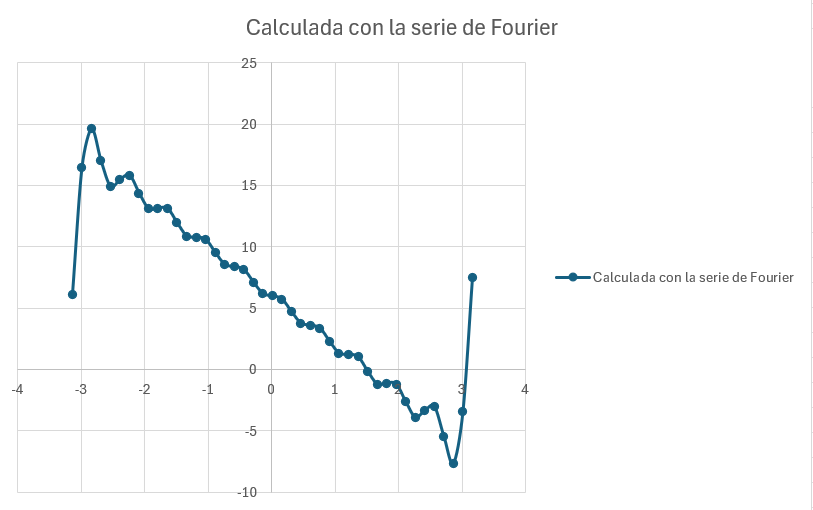
\includegraphics[width=0.9\linewidth,height=0.3\textheight]{Figures/fourierHariel/fase2/funcion_fourier.png}
        \caption[Gráfica en Excel de la función de Fourier para la función\(f(x)=6-4x\)]{Gráfica en Excel de la función de Fourier para la función \(f(x)=6-4x\), resuelto por Padilla Sanchez Hariel}
        \label{fig:figure-hariel-04}
    \end{figure}

    Finalmente, al comparar ambas gráficas en la figura (\ref{fig:figure-hariel-05}), se observa que el comportamiento de la serie de Fourier refleja fielmente la tendencia de la función f(x).Este resultado confirma que, a medida que se incluyen más términos en la suma, la precisión de la aproximación mejora significativamente.

    % Tercer Gráfica - gráficas comparativas %
    \begin{figure}[H]
        \centering
        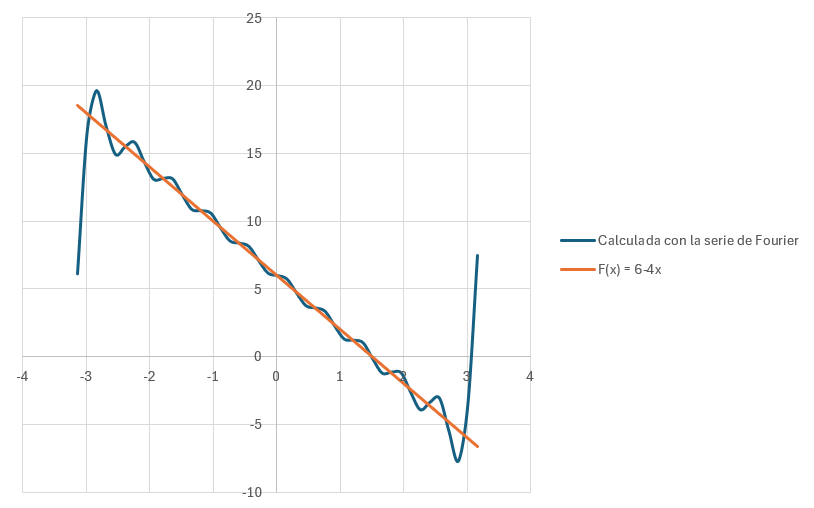
\includegraphics[width=0.9\linewidth, height=0.3\textheight]{Figures/fourierHariel/fase2/funciones_juntas.png}
        \caption[Gráfica en Excel de la función de Fourier para la función\(f(x)=6-4x\) y su función de Fourier]{Gráfica en Excel de la función de Fourier para la función \(f(x)=6-4x\) y su función de Fourier, resuelto por Padilla Sanchez Hariel}
        \label{fig:figure-hariel-05}
    \end{figure}
\end{minipage}
\clearpage
